\documentclass[11pt,letterpaper]{article}
\usepackage[utf8]{inputenc}
\usepackage[T1]{fontenc}
\usepackage{lmodern}
\usepackage[margin=1in]{geometry}
\usepackage{amsmath,amssymb,amsfonts,amsthm}
\usepackage{booktabs}
\usepackage{microtype}
\usepackage{enumitem}
\usepackage{fancyhdr}
\usepackage{titlesec}
\usepackage{xcolor}
\usepackage{tikz}
\usepackage{pgfplots}
\usepackage{mdframed}
\usepackage[hidelinks,colorlinks=true,linkcolor=SlateBlue,citecolor=SlateBlue,urlcolor=Terracotta]{hyperref}

\pgfplotsset{compat=1.18}
\usetikzlibrary{arrows.meta,positioning,calc,patterns,decorations.pathreplacing}

\definecolor{SlateBlue}{HTML}{1E293B}
\definecolor{Terracotta}{HTML}{C2410C}
\definecolor{ForestGreen}{HTML}{15803D}
\definecolor{LightSlate}{HTML}{F8FAFC}
\definecolor{BorderGray}{HTML}{CBD5E1}
\definecolor{LightTerracotta}{HTML}{FFF7ED}
\definecolor{CourseBlue}{HTML}{0072B2}
\definecolor{CourseOrange}{HTML}{D55E00}
\definecolor{CourseTeal}{HTML}{009E73}
\definecolor{CoursePurple}{HTML}{CC79A7}
\definecolor{CourseAmber}{HTML}{E69F00}

\titleformat{\section}{\normalfont\Large\bfseries\color{SlateBlue}}{\thesection}{1em}{}[\titlerule]
\titleformat{\subsection}{\normalfont\large\bfseries\color{SlateBlue}}{\thesubsection}{1em}{}
\titleformat{\subsubsection}{\normalfont\normalsize\bfseries\color{Terracotta}}{\thesubsubsection}{1em}{}

\pagestyle{fancy}
\fancyhf{}
\renewcommand{\headrulewidth}{0.4pt}
\renewcommand{\footrulewidth}{0.4pt}
\fancyhead[L]{\small\scshape\color{SlateBlue}\leftmark}
\fancyhead[R]{\small\color{SlateBlue}Principles of Economics}
\fancyfoot[C]{\thepage}

\newmdenv[
  linecolor=Terracotta,
  linewidth=1.5pt,
  backgroundcolor=LightTerracotta,
  innertopmargin=10pt,
  innerbottommargin=10pt,
  innerrightmargin=12pt,
  innerleftmargin=12pt,
  roundcorner=4pt,
  skipabove=12pt,
  skipbelow=12pt
]{coreprinciple}

\newmdenv[
  linecolor=SlateBlue,
  linewidth=1.5pt,
  backgroundcolor=LightSlate,
  innertopmargin=10pt,
  innerbottommargin=10pt,
  innerrightmargin=12pt,
  innerleftmargin=12pt,
  roundcorner=4pt,
  skipabove=12pt,
  skipbelow=12pt
]{casestudy}

\newenvironment{examplecase}[1]{%
  \begin{casestudy}
  \boxheader{SlateBlue}{#1}
  \vspace{0.4em}
}{%
  \end{casestudy}
}

\newmdenv[
  linecolor=BorderGray,
  linewidth=1pt,
  backgroundcolor=white,
  innertopmargin=10pt,
  innerbottommargin=10pt,
  innerrightmargin=12pt,
  innerleftmargin=12pt,
  roundcorner=4pt,
  skipabove=12pt,
  skipbelow=12pt
]{takeaways}

\newcommand{\boxheader}[2]{{\noindent\bfseries\color{#1}\Large #2}\vspace{0.4em}\par}

% ==============================================================================
% TikZ & PGFPlots Global Configuration and Economics Styling
% ==============================================================================

\usepackage{tikz}
\usepackage{pgfplots}
\pgfplotsset{compat=1.18}

% TikZ Libraries
\usetikzlibrary{
    arrows.meta,
    positioning,
    calc,
    shapes.geometric,
    patterns,
    decorations.pathreplacing,
    intersections
}

% Common Economics TikZ Styles
\tikzset{
    % Axes and Structural Lines
    econ axis/.style={->, >=Stealth, thick, color=SlateBlue!90!black},
    econ grid/.style={thin, dashed, color=gray!30},
    econ guide/.style={dashed, color=gray!60, thin},
    % Curves and Functions
    demand curve/.style={very thick, color=SlateBlue},
    supply curve/.style={very thick, color=Terracotta},
    mb curve/.style={very thick, color=SlateBlue},
    mc curve/.style={very thick, color=Terracotta},
    % Points and Highlights
    econ point/.style={circle, fill=SlateBlue!90!black, inner sep=1.8pt},
    econ highlight/.style={fill=Terracotta!20, opacity=0.5},
    % Annotations
    econ label/.style={font=\small\sffamily, align=center},
    econ annotation/.style={font=\footnotesize\itshape, color=SlateBlue!80!black}
}

% PGFPlots Standard Economics Style
\pgfplotsset{
    econ diagram/.style={
        axis lines=left,
        xlabel style={at={(ticklabel* cs:1)}, anchor=north west, font=\small\bfseries},
        ylabel style={at={(ticklabel* cs:1)}, anchor=south east, font=\small\bfseries},
        label style={font=\small},
        tick label style={font=\small},
        grid=none,
        enlargelimits=false,
        axis line style={->, >=Stealth, thick, color=SlateBlue!90!black}
    }
}


% Okabe-Ito Colorblind-Safe Palette Definitions (Self-Contained Guardrail)
\definecolor{oiBlue}{HTML}{0072B2}
\definecolor{oiOrange}{HTML}{D55E00}
\definecolor{oiTeal}{HTML}{009E73}
\definecolor{oiPurple}{HTML}{CC79A7}
\definecolor{oiAmber}{HTML}{E69F00}
\definecolor{oiSlate}{HTML}{1E293B}

\begin{document}

\title{\Huge\bfseries\color{SlateBlue} Chapter 9: Aggregate Demand and Aggregate Supply (AD--AS)}
\author{\large Principles of Macroeconomics Curriculum}
\date{2026}
\maketitle

\thispagestyle{plain}

\begin{abstract}
This chapter develops the Aggregate Demand--Aggregate Supply ($AD\text{--}AS$) framework to explain short-run business cycle fluctuations in real output, unemployment, and the aggregate price level alongside long-run economic growth and nominal adjustment. Aligned with Krugman and Wells's macroeconomics progression, each core topic integrates conceptual intuition, Okabe-Ito coordinate geometry, empirical U.S. Federal Reserve Economic Data (FRED) applications, and algebra-first equilibrium modeling.
\end{abstract}

\tableofcontents
\vspace{1.5em}
\hrule
\vspace{1.5em}

% ==============================================================================
% SECTION 1: LEARNING OUTCOMES, KEY TERMS & OPENING ANCHOR
% ==============================================================================
\section{Learning Outcomes, Key Terms, and Opening Dilemma}

\subsection*{Course Learning Outcomes (CLOs)}
Upon completing this chapter, students will be able to:
\begin{enumerate}
    \item Distinguish a movement along the Aggregate Demand ($AD$) curve caused by a change in the aggregate price level from a shift of the $AD$ curve caused by changes in planned spending ($C, I, G, NX$).
    \item Explain why the Short-Run Aggregate Supply ($SRAS$) curve slopes upward due to nominal wage and price stickiness, whereas the Long-Run Aggregate Supply ($LRAS$) curve is vertical at potential output ($Y^*$).
    \item Diagnose recessionary output gaps ($Y < Y^*$) and inflationary output gaps ($Y > Y^*$) using $AD\text{--}SRAS\text{--}LRAS$ equilibrium coordinates and trace the economy's long-run self-correcting adjustment.
    \item Contrast the macroeconomic effects of demand shocks with adverse supply shocks (stagflation) both graphically and algebraically, and evaluate empirical co-movements across \texttt{GDPC1}, \texttt{CPIAUCSL}, and \texttt{UNRATE}.
\end{enumerate}
\noindent\textit{Curricular Alignment:} Supports SFSU ECON 102 Course Learning Outcome \textbf{MA-3} and California C-ID \textbf{ECON 202 (C2002-2)}.

\subsection*{Key Terms}
\textbf{Aggregate Demand ($AD$)} $\bullet$ \textbf{Wealth Effect} $\bullet$ \textbf{Interest-Rate Effect} $\bullet$ \textbf{Exchange-Rate (Net Export) Effect} $\bullet$ \textbf{Short-Run Aggregate Supply ($SRAS$)} $\bullet$ \textbf{Sticky Wages and Prices} $\bullet$ \textbf{Long-Run Aggregate Supply ($LRAS$)} $\bullet$ \textbf{Potential Output ($Y^*$)} $\bullet$ \textbf{Recessionary Gap} $\bullet$ \textbf{Inflationary Gap} $\bullet$ \textbf{Self-Correcting Mechanism} $\bullet$ \textbf{Demand Shock} $\bullet$ \textbf{Supply Shock} $\bullet$ \textbf{Stagflation}.

\begin{coreprinciple}
\boxheader{SlateBlue}{Bring It Home: Why Did 2021--2023 Combine High Inflation with Shifting Output?}
In 2020, pandemic lockdowns caused total spending and production to plunge simultaneously. By 2021--2022, aggressive fiscal stimulus and pent-up household demand collided with global semiconductor shortages, port bottlenecks, and a sharp spike in global energy prices following geopolitical conflict. Consumer price inflation (\texttt{CPIAUCSL}) surged to a four-decade high above 9\%, while policymakers debated whether rising prices reflected excessive aggregate demand or constrained aggregate supply. The $AD\text{--}AS$ model provides the exact analytical lens required to separate demand-driven expansions from supply-driven stagflation.
\end{coreprinciple}

% ==============================================================================
% SECTION 2: AGGREGATE DEMAND (AD)
% ==============================================================================
\section{Aggregate Demand: Total Planned Spending and the Price Level}

\subsection{Conceptual Introduction}
\textbf{Aggregate Demand ($AD$)} represents the total quantity of domestically produced final goods and services that households, firms, governments, and foreign buyers plan to purchase at each aggregate price level ($P$), holding all non-price determinants constant (\textit{ceteris paribus}). Summing across the four expenditure sectors established in Chapter 4 gives total planned spending:
\[
AD = C + I + G + NX
\]
Unlike a microeconomic demand curve—which holds all other prices and consumer income constant while varying the relative price of a single good—the $AD$ curve tracks economy-wide real output ($Y$) as the overall price level ($P$, measured by the GDP deflator or CPI) changes across all markets simultaneously.

Three distinct macroeconomic channels explain why the $AD$ curve slopes downward from left to right:
\begin{enumerate}
    \item \textbf{The Wealth (Real-Balances) Effect:} When the aggregate price level $P$ falls, the real purchasing power of households' fixed nominal financial assets (cash, checking deposits, nominal bonds) rises. Feeling wealthier, households increase real consumption spending ($C$).
    \item \textbf{The Interest-Rate Effect:} A lower price level reduces the amount of money households and firms need to hold for everyday transactions. As money demand falls, nominal and real interest rates ($r$) decline, lowering borrowing costs and stimulating business investment ($I$) and durable consumption ($C$).
    \item \textbf{The Exchange-Rate (Net Export) Effect:} When lower domestic interest rates reduce the return on U.S. financial assets relative to foreign assets, capital outflows depreciate the domestic currency. A weaker currency makes domestic exports cheaper for foreign buyers and imports more expensive for domestic residents, increasing net exports ($NX = X - M$).
\end{enumerate}

When any factor \emph{other than} the current domestic price level alters planned spending at every price level, the entire $AD$ curve shifts. Rightward shifts ($AD_1 \rightarrow AD_2$) result from stronger consumer confidence, higher expected business profitability, expansionary fiscal policy (higher $G$ or lower taxes $T$), expansionary monetary policy (lower policy interest rates), faster foreign GDP growth, or currency depreciation. Leftward shifts occur when these forces reverse.

\subsection{Visual Representation}
\begin{figure}[htbp]
\centering
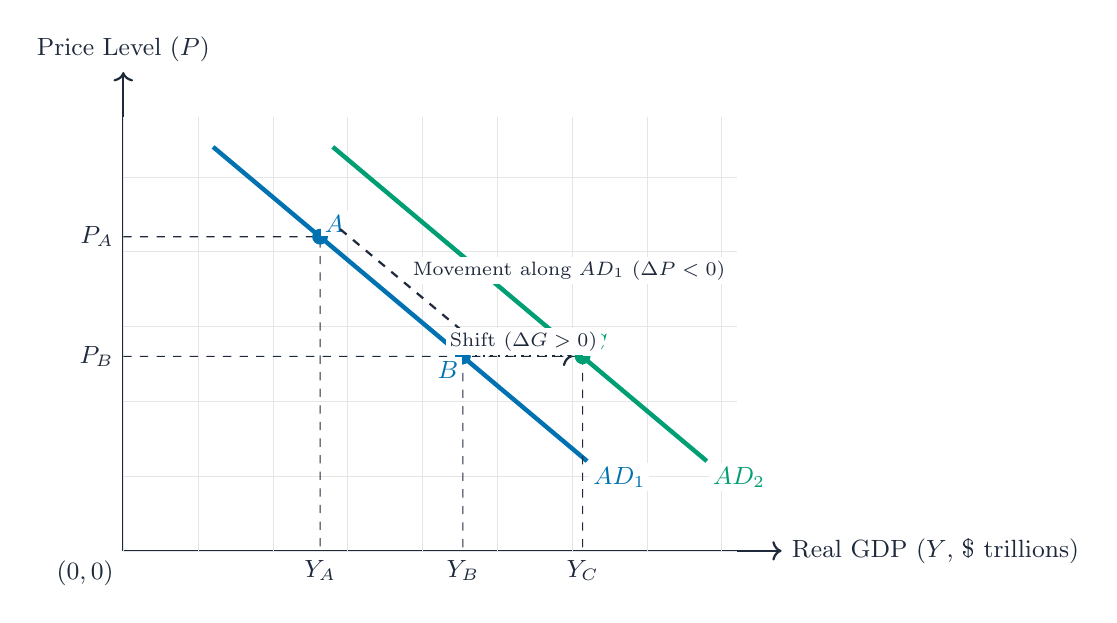
\begin{tikzpicture}[scale=0.95]
    % Axes
    \draw[->, thick, oiSlate] (0,0) -- (8.8,0) node[right] {\small Real GDP ($Y$, \$ trillions)};
    \draw[->, thick, oiSlate] (0,0) -- (0,6.4) node[above] {\small Price Level ($P$)};
    \node[below left, oiSlate] at (0,0) {\small $(0,0)$};

    % Grid (subtle)
    \draw[very thin, gray!20] (0,0) grid (8.2,5.8);

    % AD1 (Baseline) and AD2 (Rightward Shift)
    \draw[ultra thick, oiBlue] (1.2,5.4) -- (6.2,1.2) node[below right, fill=white, inner sep=1.5pt] {\small $AD_1$};
    \draw[ultra thick, oiTeal] (2.8,5.4) -- (7.8,1.2) node[below right, fill=white, inner sep=1.5pt] {\small $AD_2$};

    % Points A and B on AD1 (Movement along AD)
    \coordinate (A) at (2.63,4.2);
    \coordinate (B) at (4.54,2.6);
    \coordinate (Cpt) at (6.14,2.6);

    % Projection Drop-lines
    \draw[dashed, oiSlate] (0,4.2) node[left] {\small $P_A$} -- (A) -- (2.63,0) node[below] {\small $Y_A$};
    \draw[dashed, oiSlate] (0,2.6) node[left] {\small $P_B$} -- (Cpt);
    \draw[dashed, oiSlate] (B) -- (4.54,0) node[below] {\small $Y_B$};
    \draw[dashed, oiSlate] (Cpt) -- (6.14,0) node[below] {\small $Y_C$};

    % Plot Points
    \fill[oiBlue] (A) circle (3pt) node[above right, fill=white, inner sep=1.5pt] {\small $A$};
    \fill[oiBlue] (B) circle (3pt) node[below left, fill=white, inner sep=1.5pt] {\small $B$};
    \fill[oiTeal] (Cpt) circle (3pt) node[above right, fill=white, inner sep=1.5pt] {\small $C$};

    % Callout Arrows (Dashed/Dotted Slate per Visualization Rules)
    \draw[->, thick, dashed, oiSlate] (2.9,4.3) -- (4.7,2.8) node[midway, above right, fill=white, inner sep=1.5pt, font=\scriptsize] {Movement along $AD_1$ ($\Delta P < 0$)};
    \draw[->, thick, dotted, oiSlate] (4.7,2.6) -- (6.0,2.6) node[midway, above, fill=white, inner sep=1.5pt, font=\scriptsize] {Shift ($\Delta G > 0$)};
\end{tikzpicture}
\caption{\textbf{Reading the $AD$ Curve:} A lower price level ($P_A \rightarrow P_B$) induces a movement along $AD_1$ from point $A$ to point $B$ ($Y_A \rightarrow Y_B$), whereas an autonomous spending surge at constant price level $P_B$ shifts the entire curve rightward from $AD_1$ to $AD_2$ (point $B$ to point $C$).}
\label{fig:ad_movement_vs_shift}
\end{figure}

\subsection{Real-World Application}
\textbf{Interest-Rate Sensitivity in U.S. Residential Investment (2022--2024):} When the Federal Reserve raised its administered interest-rate corridor during 2022--2023 to curb post-pandemic inflation, 30-year fixed mortgage rates rose from roughly 3\% to over 7\%. Even before overall consumer prices fell, higher borrowing costs sharply reduced planned residential investment ($I$) and auto/durable purchases ($C$), shifting the U.S. $AD$ curve leftward relative to its 2021 trajectory and cooling excess demand.

\begin{coreprinciple}
\boxheader{SlateBlue}{Clear It Up: Movement Along $AD$ vs. Shift of $AD$}
A change in the domestic aggregate price level $P$ causes a \textbf{movement along} a stationary $AD$ curve via the wealth, interest-rate, and exchange-rate effects. By contrast, a change in autonomous consumption, investment, government purchases, net exports, or monetary/fiscal policy at any \emph{given} price level \textbf{shifts} the entire $AD$ curve. Never treat an endogenous change in $P$ as a shifter of $AD$.
\end{coreprinciple}

\subsection{Mathematical Foundation}
Assume linear aggregate planned expenditure where autonomous spending responds inversely to the price level $P$ (capturing the wealth, interest-rate, and exchange-rate channels with slope parameter $\beta > 0$):
\[
AD: \quad Y = A_0 - \beta P \qquad \Longleftrightarrow \qquad P = \frac{A_0}{\beta} - \frac{1}{\beta} Y
\]
Here, $A_0$ summarizes non-price autonomous spending determinants ($C_0, I_0, G, NX_0$). Any increase $\Delta A_0 > 0$ shifts the horizontal intercept rightward by $\Delta Y = \Delta A_0$ at every price level $P$.

\begin{examplecase}{Work It Out: Quantifying a Movement Along $AD$ vs. a Fiscal Shift}
Suppose baseline Aggregate Demand is given by $Y = 45 - 0.25P$ (with $Y$ in trillions of 2017 dollars and $P$ as a price index).
\begin{enumerate}
    \item \textbf{Movement Along $AD$:} Calculate real output demanded when $P = 120$ versus $P = 100$.
    \begin{itemize}
        \item At $P = 120$: $Y_A = 45 - 0.25(120) = 45 - 30 = \$15.0\text{ trillion}$.
        \item At $P = 100$: $Y_B = 45 - 0.25(100) = 45 - 25 = \$20.0\text{ trillion}$.
        \item Moving from $P = 120$ to $P = 100$ expands quantity demanded by $+\$5.0\text{ trillion}$ along the same curve.
    \end{itemize}
    \item \textbf{Shift of $AD$:} Suppose an autonomous investment boom increases $A_0$ by $\$4.0\text{ trillion}$ at every price level, yielding $Y = 49 - 0.25P$. At $P = 100$:
    \[
    Y_C = 49 - 0.25(100) = 49 - 25 = \$24.0\text{ trillion}
    \]
    At an unchanged price level of $P = 100$, the $AD$ curve shifts horizontally rightward by $\Delta Y = \$4.0\text{ trillion}$.
\end{enumerate}
\end{examplecase}

% ==============================================================================
% SECTION 3: SHORT-RUN AND LONG-RUN AGGREGATE SUPPLY (SRAS & LRAS)
% ==============================================================================
\section{Short-Run and Long-Run Aggregate Supply}

\subsection{Conceptual Introduction}
\textbf{Aggregate Supply} links the aggregate price level ($P$) to the total quantity of real goods and services ($Y$) that domestic firms are willing and able to produce. Crucially, supply behavior depends on the time horizon over which input costs adjust:
\begin{itemize}
    \item \textbf{Short-Run Aggregate Supply ($SRAS$):} In the short run, nominal wages and many input prices are \emph{sticky}—locked in by multi-year union contracts, annual salary cycles, or menu costs. When the overall price level $P$ rises while nominal unit production costs remain temporarily fixed, revenue per unit rises faster than cost per unit. Profit margins widen, inducing firms to expand production and hire more workers, which gives $SRAS$ its positive upward slope.
    \item \textbf{Long-Run Aggregate Supply ($LRAS$):} In the long run, all nominal wages, input prices, and price expectations adjust fully to match the aggregate price level. Because doubling all output prices and all input wages leaves real relative prices and profit margins unchanged, long-run output is independent of $P$. Consequently, $LRAS$ is vertical at \textbf{potential output ($Y^*$)}—the sustainable level of real GDP determined by the economy's labor force, physical and human capital stock, natural resources, technology, and institutions (corresponding to the natural rate of unemployment $u^*$).
\end{itemize}

While $LRAS$ shifts rightward over decades through capital deepening, labor force growth, and technological innovation (mirroring outward shifts of the Macroeconomic PPF in Chapter 2), $SRAS$ shifts whenever unit production costs or price expectations change:
\begin{enumerate}
    \item \textbf{Nominal Wage Changes:} Higher nominal wage settlements raise unit labor costs and shift $SRAS$ leftward (upward).
    \item \textbf{Commodity and Energy Prices:} Spikes in oil, electricity, or raw material prices raise production costs and shift $SRAS$ leftward.
    \item \textbf{Expected Price Level ($P^e$):} When workers and firms expect higher inflation ($P^e \uparrow$), they negotiate higher nominal wages today, shifting $SRAS$ leftward.
    \item \textbf{Productivity Shocks:} Advances in total factor productivity lower unit costs and shift both $SRAS$ and $LRAS$ rightward.
\end{enumerate}

\subsection{Visual Representation}
\begin{figure}[htbp]
\centering
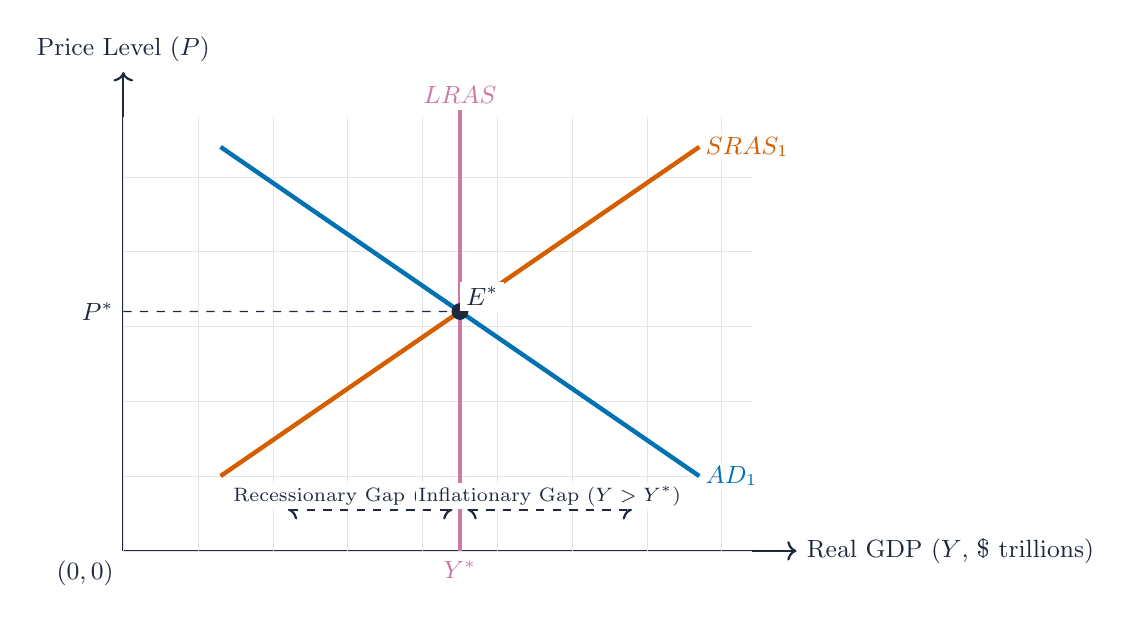
\begin{tikzpicture}[scale=0.95]
    % Axes
    \draw[->, thick, oiSlate] (0,0) -- (9.0,0) node[right] {\small Real GDP ($Y$, \$ trillions)};
    \draw[->, thick, oiSlate] (0,0) -- (0,6.4) node[above] {\small Price Level ($P$)};
    \node[below left, oiSlate] at (0,0) {\small $(0,0)$};
    \draw[very thin, gray!20] (0,0) grid (8.4,5.8);

    % LRAS at Y* = 4.5
    \draw[ultra thick, oiPurple] (4.5,0) -- (4.5,5.9) node[above, fill=white, inner sep=1.5pt] {\small $LRAS$};
    \node[below, oiPurple] at (4.5,0) {\small $Y^*$};

    % SRAS1 and AD1 intersecting at E* = (4.5, 3.2)
    \draw[ultra thick, oiOrange] (1.3,1.0) -- (7.7,5.4) node[right, fill=white, inner sep=1.5pt] {\small $SRAS_1$};
    \draw[ultra thick, oiBlue] (1.3,5.4) -- (7.7,1.0) node[right, fill=white, inner sep=1.5pt] {\small $AD_1$};

    % Equilibrium E*
    \coordinate (Estar) at (4.5,3.2);
    \draw[dashed, oiSlate] (0,3.2) node[left] {\small $P^*$} -- (Estar);
    \fill[oiSlate] (Estar) circle (3.2pt) node[above right, fill=white, inner sep=2pt] {\small $E^*$};

    % Annotate Recessionary vs Inflationary Gap Zones cleanly below axis
    \draw[<->, thick, dashed, oiSlate] (2.2,0.55) -- (4.4,0.55) node[midway, above, fill=white, inner sep=1pt, font=\scriptsize] {Recessionary Gap ($Y < Y^*$)};
    \draw[<->, thick, dashed, oiSlate] (4.6,0.55) -- (6.8,0.55) node[midway, above, fill=white, inner sep=1pt, font=\scriptsize] {Inflationary Gap ($Y > Y^*$)};
\end{tikzpicture}
\caption{\textbf{Macroeconomic Equilibrium and Output Gaps:} Long-run equilibrium occurs at $E^*$ where $AD_1$, $SRAS_1$, and vertical $LRAS$ intersect at $(Y^*, P^*)$. Short-run equilibria to the left of $Y^*$ create recessionary gaps ($u > u^*$), whereas equilibria to the right of $Y^*$ create inflationary gaps ($u < u^*$).}
\label{fig:lras_sras_equilibrium}
\end{figure}

\subsection{Real-World Application}
\textbf{AI Infrastructure, Productivity, and $LRAS$ vs. $SRAS$:} Heavy capital investment in data centers, automation, and cloud computing initially boosts $AD$ through higher business investment ($I$). Over a multi-year horizon, however, if those technologies raise output per worker across logistics, healthcare, and software, they reduce unit labor costs—shifting both $SRAS$ and vertical $LRAS$ rightward and allowing higher non-inflationary potential output ($Y^*$).

\subsection{Mathematical Foundation}
In linear form, Short-Run Aggregate Supply reflects sticky nominal wages ($W_0$) anchored to the expected price level ($P^e$) with supply slope parameter $\gamma > 0$:
\[
SRAS: \quad Y = Y^* + \gamma (P - P^e) \qquad \Longleftrightarrow \qquad P = P^e + \frac{1}{\gamma}(Y - Y^*)
\]
When actual prices equal expected prices ($P = P^e$), short-run output equals potential output ($Y = Y^*$), which defines the vertical $LRAS$ schedule. If $P > P^e$, real wages ($W_0 / P$) fall temporarily and firms expand output above $Y^*$; if $P < P^e$, real wages rise and firms cut production below $Y^*$.

% ==============================================================================
% SECTION 4: DEMAND SHOCKS, SUPPLY SHOCKS & LONG-RUN SELF-CORRECTION
% ==============================================================================
\section{Demand Shocks, Stagflation, and Long-Run Adjustment}

\subsection{Conceptual Introduction}
Macroeconomic fluctuations arise from exogenous \textbf{shocks} that displace the economy from $E^* = (Y^*, P^*)$:
\begin{enumerate}
    \item \textbf{Positive Demand Shock ($AD_1 \rightarrow AD_2$) and Self-Correction:} A surge in planned spending raises both short-run output ($Y_2 > Y^*$) and the price level ($P_2 > P^*$), opening an \textbf{inflationary gap} where unemployment falls below $u^*$. Because labor markets are tight and workers' real purchasing power has been eroded by higher prices ($P_2 > P^e$), workers demand higher nominal wages as contracts renew. Rising nominal wages increase unit production costs, shifting $SRAS$ leftward ($SRAS_1 \rightarrow SRAS_2$) until output returns to $Y^*$ at a permanently higher price level ($P_3 > P_2$). Conversely, after a negative demand shock creates a recessionary gap ($Y < Y^*$), high unemployment eventually puts downward pressure on nominal wage growth, shifting $SRAS$ rightward back to $Y^*$—though downward nominal wage stickiness often makes self-correction from recessions slow and painful.
    \item \textbf{Adverse Supply Shock ($SRAS_1 \rightarrow SRAS_2$) and Stagflation:} A sharp spike in energy or commodity costs shifts $SRAS$ leftward. In the short run, real output falls ($Y_2 < Y^*$, raising unemployment) while the price level rises ($P_2 > P^*$). This combination of economic stagnation and rising inflation is called \textbf{stagflation}. Unlike demand shocks—where output and prices move in the \emph{same} direction—supply shocks push output and prices in \emph{opposite} directions, creating a painful policy dilemma because stimulating $AD$ fights unemployment at the cost of even higher inflation.
\end{enumerate}

\subsection{Visual Representation}
\begin{figure}[htbp]
\centering
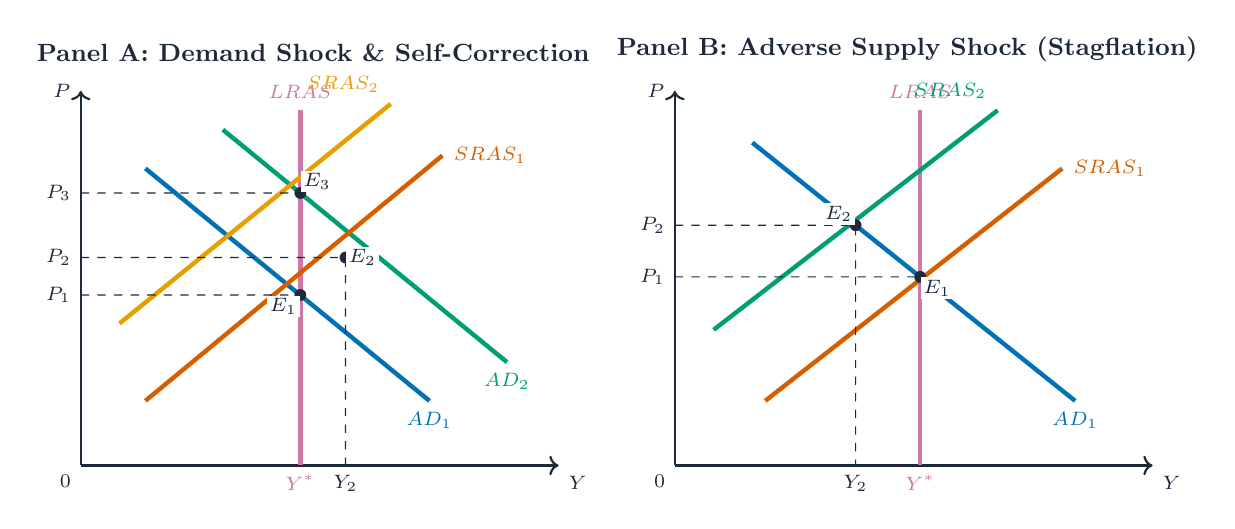
\begin{tikzpicture}[scale=0.82]
    % Panel A: Demand Shock + Self-Correction
    \begin{scope}[shift={(0,0)}]
        \node[above, font=\bfseries\small, oiSlate] at (3.6,6.1) {Panel A: Demand Shock \& Self-Correction};
        \draw[->, thick, oiSlate] (0,0) -- (7.4,0) node[below right] {\scriptsize $Y$};
        \draw[->, thick, oiSlate] (0,0) -- (0,5.8) node[left] {\scriptsize $P$};
        \node[below left, oiSlate] at (0,0) {\scriptsize $0$};

        \draw[ultra thick, oiPurple] (3.4,0) -- (3.4,5.5) node[above] {\scriptsize $LRAS$};
        \node[below, oiPurple] at (3.4,0) {\scriptsize $Y^*$};

        \draw[ultra thick, oiBlue] (1.0,4.6) -- (5.4,1.0) node[below] {\scriptsize $AD_1$};
        \draw[ultra thick, oiTeal] (2.2,5.2) -- (6.6,1.6) node[below] {\scriptsize $AD_2$};

        \draw[ultra thick, oiOrange] (1.0,1.0) -- (5.6,4.8) node[right] {\scriptsize $SRAS_1$};
        \draw[ultra thick, oiAmber] (0.6,2.2) -- (4.8,5.6) node[above left] {\scriptsize $SRAS_2$};

        \coordinate (E1) at (3.4,2.64);
        \coordinate (E2) at (4.1,3.22);
        \coordinate (E3) at (3.4,4.22);

        \draw[dashed, oiSlate] (0,2.64) node[left] {\scriptsize $P_1$} -- (E1);
        \draw[dashed, oiSlate] (0,3.22) node[left] {\scriptsize $P_2$} -- (E2) -- (4.1,0) node[below] {\scriptsize $Y_2$};
        \draw[dashed, oiSlate] (0,4.22) node[left] {\scriptsize $P_3$} -- (E3);

        \fill[oiSlate] (E1) circle (2.6pt) node[below left, fill=white, inner sep=1pt] {\scriptsize $E_1$};
        \fill[oiSlate] (E2) circle (2.6pt) node[right, fill=white, inner sep=1pt] {\scriptsize $E_2$};
        \fill[oiSlate] (E3) circle (2.6pt) node[above right, fill=white, inner sep=1pt] {\scriptsize $E_3$};
    \end{scope}

    % Panel B: Adverse Supply Shock (Stagflation)
    \begin{scope}[shift={(9.2,0)}]
        \node[above, font=\bfseries\small, oiSlate] at (3.6,6.1) {Panel B: Adverse Supply Shock (Stagflation)};
        \draw[->, thick, oiSlate] (0,0) -- (7.4,0) node[below right] {\scriptsize $Y$};
        \draw[->, thick, oiSlate] (0,0) -- (0,5.8) node[left] {\scriptsize $P$};
        \node[below left, oiSlate] at (0,0) {\scriptsize $0$};

        \draw[ultra thick, oiPurple] (3.8,0) -- (3.8,5.5) node[above] {\scriptsize $LRAS$};
        \node[below, oiPurple] at (3.8,0) {\scriptsize $Y^*$};

        \draw[ultra thick, oiBlue] (1.2,5.0) -- (6.2,1.0) node[below] {\scriptsize $AD_1$};
        \draw[ultra thick, oiOrange] (1.4,1.0) -- (6.0,4.6) node[right] {\scriptsize $SRAS_1$};
        \draw[ultra thick, oiTeal] (0.6,2.1) -- (5.0,5.5) node[above left] {\scriptsize $SRAS_2$};

        \coordinate (S1) at (3.8,2.92);
        \coordinate (S2) at (2.8,3.72);

        \draw[dashed, oiSlate] (0,2.92) node[left] {\scriptsize $P_1$} -- (S1);
        \draw[dashed, oiSlate] (0,3.72) node[left] {\scriptsize $P_2$} -- (S2) -- (2.8,0) node[below] {\scriptsize $Y_2$};

        \fill[oiSlate] (S1) circle (2.6pt) node[below right, fill=white, inner sep=1pt] {\scriptsize $E_1$};
        \fill[oiSlate] (S2) circle (2.6pt) node[above left, fill=white, inner sep=1pt] {\scriptsize $E_2$};
    \end{scope}
\end{tikzpicture}
\caption{\textbf{Comparing Demand and Supply Shocks:} In Panel A, a positive demand shock moves the economy from $E_1$ to $E_2$ ($Y_2 > Y^*$, $P_2 > P_1$), followed by rising nominal wages shifting $SRAS_1 \rightarrow SRAS_2$ to long-run equilibrium $E_3$ at $Y^*$. In Panel B, an adverse supply shock shifts $SRAS_1 \rightarrow SRAS_2$, reducing output ($Y_2 < Y^*$) while raising the price level ($P_2 > P_1$).}
\label{fig:shocks_comparison}
\end{figure}

\subsection{Real-World Application}
\begin{examplecase}{FRED Data Diagnostics: Identifying Shocks Across \texttt{GDPC1}, \texttt{CPIAUCSL}, and \texttt{UNRATE}}
Macroeconomists track three canonical St. Louis Fed FRED series to diagnose historical episodes:
\begin{itemize}
    \item \texttt{GDPC1}: Real Gross Domestic Product (billions of chained 2017 dollars, quarterly, seasonally adjusted annual rate).
    \item \texttt{CPIAUCSL}: Consumer Price Index for All Urban Consumers: All Items (index $1982\text{--}1984 = 100$, monthly, seasonally adjusted).
    \item \texttt{UNRATE}: Civilian Unemployment Rate (percent, monthly, seasonally adjusted).
\end{itemize}
\textbf{Empirical Identification Rule:} During the 2008--2009 Great Recession, \texttt{GDPC1} contracted while \texttt{CPIAUCSL} decelerated/dipped and \texttt{UNRATE} surged toward 10\%—the classic signature of an adverse \textbf{demand shock}. Conversely, during the 1973--1975 and 1979--1980 OPEC oil embargoes, \texttt{GDPC1} fell and \texttt{UNRATE} jumped while \texttt{CPIAUCSL} inflation exceeded 11\%—the unmistakable empirical footprint of an adverse \textbf{supply shock (stagflation)}. Because monthly price series (\texttt{CPIAUCSL}) and quarterly output series (\texttt{GDPC1}) differ in frequency and undergo statistical revisions, structural identification requires examining relative input prices alongside aggregate movements.
\end{examplecase}

\subsection{Mathematical Foundation (Algebra-First with Optional Calculus Box)}

\begin{examplecase}{Work It Out: Complete Equilibrium, Demand Shock, Self-Correction, and Stagflation}
Consider an economy described by the following linear schedules ($Y$ in trillions of chained 2017 dollars, $P$ as price index):
\[
AD_1: \; P = 180 - 4Y \qquad\qquad SRAS_1: \; P = 20 + 4Y \qquad\qquad LRAS: \; Y^* = 20
\]
\textbf{Part A: Initial Long-Run Equilibrium ($E_1$)} \\
Set $AD_1 = SRAS_1$:
\[
180 - 4Y = 20 + 4Y \implies 160 = 8Y \implies Y_1 = 20
\]
Substitute $Y_1 = 20$ into $AD_1$: $P_1 = 180 - 4(20) = 100$. Since $Y_1 = Y^* = 20$, the economy begins in long-run equilibrium at $(Y^* = 20, P_1 = 100)$.

\medskip
\noindent\textbf{Part B: Positive Demand Shock ($AD_1 \rightarrow AD_2$) and Output Gap} \\
Suppose a surge in business investment shifts $AD$ to $AD_2: \; P = 196 - 4Y$. Equate $AD_2 = SRAS_1$:
\[
196 - 4Y = 20 + 4Y \implies 176 = 8Y \implies Y_2 = 22
\]
Substitute $Y_2 = 22$ into $AD_2$: $P_2 = 196 - 4(22) = 108$. \\
The economy experiences an \textbf{inflationary gap} of $Y_2 - Y^* = 22 - 20 = +\$2.0\text{ trillion}$ ($+10\%$ above potential), and the price level rises by $8\%$.

\medskip
\noindent\textbf{Part C: Long-Run Self-Correction ($SRAS_1 \rightarrow SRAS_2$)} \\
Tight labor markets bid up nominal wages until output returns to $Y_3 = Y^* = 20$ along $AD_2$:
\[
P_3 = 196 - 4(20) = 116
\]
The new short-run supply curve shifts upward by $\Delta P = +16$ to $SRAS_2: \; P = 36 + 4Y$. In the long run, real output returns to $Y^* = 20$ while the price level settles permanently at $P_3 = 116$.

\medskip
\noindent\textbf{Part D: Adverse Supply Shock / Stagflation ($SRAS_1 \rightarrow SRAS_{\text{shock}}$)} \\
Return to initial equilibrium $E_1 = (20, 100)$ on $AD_1$ ($P = 180 - 4Y$). Suppose an energy price spike shifts short-run supply upward by $16$ index points to $SRAS_{\text{shock}}: \; P = 36 + 4Y$. Equate $AD_1 = SRAS_{\text{shock}}$:
\[
180 - 4Y = 36 + 4Y \implies 144 = 8Y \implies Y_{\text{stag}} = 18
\]
Substitute $Y_{\text{stag}} = 18$ into $AD_1$: $P_{\text{stag}} = 180 - 4(18) = 108$. \\
Output falls by $\$2.0\text{ trillion}$ (a recessionary gap of $-\$2.0\text{ trillion}$) while the price level simultaneously rises from $100$ to $108$.
\end{examplecase}

\begin{coreprinciple}
\boxheader{SlateBlue}{Optional Advanced Extension: Comparative Statics via Total Differentiation}
For quantitative economics majors, consider a general differentiable short-run system:
\[
AD: \; Y = D(P, G) \quad (D_P < 0, \; D_G > 0) \qquad\text{and}\qquad SRAS: \; P = S(Y, W_0) \quad (S_Y > 0, \; S_{W_0} > 0)
\]
Taking total differentials holding nominal wages $W_0$ fixed ($dW_0 = 0$) in the short run:
\[
dY = D_P \, dP + D_G \, dG \qquad\text{and}\qquad dP = S_Y \, dY
\]
Substituting $dP = S_Y \, dY$ into the $AD$ differential yields the short-run fiscal output and price multipliers:
\[
\frac{dY}{dG} = \frac{D_G}{1 - D_P S_Y} \qquad\text{and}\qquad \frac{dP}{dG} = \frac{S_Y D_G}{1 - D_P S_Y}
\]
Because $D_P < 0$ and $S_Y > 0$, the denominator $1 - D_P S_Y > 1$. Thus, an upward-sloping $SRAS$ curve ($S_Y > 0$) dampens the short-run output multiplier relative to the fixed-price Keynesian Cross ($S_Y = 0 \Rightarrow \frac{dY}{dG} = D_G$) by crowding out price-sensitive spending as $P$ rises. In the long run, as $S_Y \rightarrow \infty$ along vertical $LRAS$, $\lim_{S_Y \to \infty} \frac{dY}{dG} = 0$ and $\lim_{S_Y \to \infty} \frac{dP}{dG} = -\frac{D_G}{D_P} > 0$.
\end{coreprinciple}

% ==============================================================================
% SECTION 5: CLOSING ANCHOR & CHECK YOUR UNDERSTANDING
% ==============================================================================
\begin{coreprinciple}
\boxheader{SlateBlue}{Bring It Home: Resolving the 2021--2023 Inflation Puzzle}
Applying the $AD\text{--}AS$ framework reveals that 2021--2023 combined \emph{both} shocks simultaneously: expansionary demand shifted $AD$ rightward (pushing output up and unemployment down toward 3.4\%), while supply-chain bottlenecks and energy spikes shifted $SRAS$ leftward. Both shifts pushed the price level $P$ upward in the same direction, explaining why inflation surged dramatically even as real GDP recovery moderated.
\end{coreprinciple}

\section{Check Your Understanding}
\begin{enumerate}
    \item \textbf{Conceptual Mechanism:} Explain how a lower domestic aggregate price level increases real output demanded through the interest-rate and exchange-rate effects without shifting the $AD$ curve.
    \item \textbf{Directional Diagnostics:} If households become more optimistic about future income and raise planned consumption at every price level, does this cause a movement along $AD$ or a shift? What happens to $Y$ and $P$ in the short run?
    \item \textbf{Supply Shock Identification:} Why does an adverse $SRAS$ shock create a policy dilemma for central banks and fiscal authorities that a negative $AD$ shock does not?
    \item \textbf{Algebraic Equilibrium:} Suppose $AD: P = 150 - 3Y$, $SRAS: P = 30 + 3Y$, and $LRAS: Y^* = 20$. Solve for initial $(Y_1, P_1)$. If an adverse supply shock shifts $SRAS$ to $P = 42 + 3Y$, calculate the new short-run equilibrium $(Y_2, P_2)$ and the resulting output gap.
    \item \textbf{Long-Run Self-Correction:} Starting from a recessionary gap where $Y_1 = 18 < Y^* = 20$, trace how falling nominal wage growth restores long-run equilibrium in the $AD\text{--}AS$ diagram.
    \item \textbf{FRED Empirical Reasoning:} Why can co-movement between \texttt{GDPC1} and \texttt{CPIAUCSL} alone not prove whether a historical business cycle was driven by a demand shock or a supply shock?
\end{enumerate}

\subsection*{Solutions}
\begin{enumerate}
    \item A lower price level reduces transactions money demand, lowering domestic interest rates ($r \downarrow$). Lower $r$ stimulates domestic business investment ($I \uparrow$) and triggers capital outflows that depreciate the currency, boosting net exports ($NX \uparrow$). Because both effects are triggered endogenously by $\Delta P < 0$, they represent a downward movement along a stationary $AD$ curve.
    \item It causes a \textbf{rightward shift of $AD$}. In the short run, the economy moves up along $SRAS$, raising both real output ($Y \uparrow$) and the price level ($P \uparrow$).
    \item A negative $AD$ shock lowers both $Y$ and $P$, so expansionary policy can simultaneously close the recessionary gap and stabilize prices. An adverse $SRAS$ shock (stagflation) lowers $Y$ while raising $P$: stimulating $AD$ reduces unemployment at the cost of worsening inflation, whereas tightening $AD$ curbs inflation at the cost of a deeper recession.
    \item Initial equilibrium: $150 - 3Y = 30 + 3Y \implies 120 = 6Y \implies Y_1 = 20$, and $P_1 = 150 - 3(20) = 90$. After the supply shock: $150 - 3Y = 42 + 3Y \implies 108 = 6Y \implies Y_2 = 18$, and $P_2 = 150 - 3(18) = 96$. The economy has a recessionary output gap of $Y_2 - Y^* = 18 - 20 = -\$2.0\text{ trillion}$.
    \item Persistent unemployment above $u^*$ gradually reduces nominal wage growth and unit production costs, shifting $SRAS$ rightward (downward) along $AD$ until output rises back to $Y^* = 20$ at a lower equilibrium price level.
    \item In a demand shock, \texttt{GDPC1} and \texttt{CPIAUCSL} move in the \emph{same} direction; in a supply shock, they move in \emph{opposite} directions. However, when simultaneous demand and supply shocks occur (or when quarterly vs. monthly frequencies and data revisions obscure timing), observational co-movement alone cannot isolate causal magnitudes without a structural identification strategy.
\end{enumerate}

\end{document}